% Options for packages loaded elsewhere
% Options for packages loaded elsewhere
\PassOptionsToPackage{unicode}{hyperref}
\PassOptionsToPackage{hyphens}{url}
\PassOptionsToPackage{dvipsnames,svgnames,x11names}{xcolor}
%
\documentclass[
  letterpaper,
  DIV=11,
  numbers=noendperiod]{scrartcl}
\usepackage{xcolor}
\usepackage{amsmath,amssymb}
\setcounter{secnumdepth}{-\maxdimen} % remove section numbering
\usepackage{iftex}
\ifPDFTeX
  \usepackage[T1]{fontenc}
  \usepackage[utf8]{inputenc}
  \usepackage{textcomp} % provide euro and other symbols
\else % if luatex or xetex
  \usepackage{unicode-math} % this also loads fontspec
  \defaultfontfeatures{Scale=MatchLowercase}
  \defaultfontfeatures[\rmfamily]{Ligatures=TeX,Scale=1}
\fi
\usepackage{lmodern}
\ifPDFTeX\else
  % xetex/luatex font selection
\fi
% Use upquote if available, for straight quotes in verbatim environments
\IfFileExists{upquote.sty}{\usepackage{upquote}}{}
\IfFileExists{microtype.sty}{% use microtype if available
  \usepackage[]{microtype}
  \UseMicrotypeSet[protrusion]{basicmath} % disable protrusion for tt fonts
}{}
\makeatletter
\@ifundefined{KOMAClassName}{% if non-KOMA class
  \IfFileExists{parskip.sty}{%
    \usepackage{parskip}
  }{% else
    \setlength{\parindent}{0pt}
    \setlength{\parskip}{6pt plus 2pt minus 1pt}}
}{% if KOMA class
  \KOMAoptions{parskip=half}}
\makeatother
% Make \paragraph and \subparagraph free-standing
\makeatletter
\ifx\paragraph\undefined\else
  \let\oldparagraph\paragraph
  \renewcommand{\paragraph}{
    \@ifstar
      \xxxParagraphStar
      \xxxParagraphNoStar
  }
  \newcommand{\xxxParagraphStar}[1]{\oldparagraph*{#1}\mbox{}}
  \newcommand{\xxxParagraphNoStar}[1]{\oldparagraph{#1}\mbox{}}
\fi
\ifx\subparagraph\undefined\else
  \let\oldsubparagraph\subparagraph
  \renewcommand{\subparagraph}{
    \@ifstar
      \xxxSubParagraphStar
      \xxxSubParagraphNoStar
  }
  \newcommand{\xxxSubParagraphStar}[1]{\oldsubparagraph*{#1}\mbox{}}
  \newcommand{\xxxSubParagraphNoStar}[1]{\oldsubparagraph{#1}\mbox{}}
\fi
\makeatother


\usepackage{longtable,booktabs,array}
\newcounter{none} % for unnumbered tables
\usepackage{calc} % for calculating minipage widths
% Correct order of tables after \paragraph or \subparagraph
\usepackage{etoolbox}
\makeatletter
\patchcmd\longtable{\par}{\if@noskipsec\mbox{}\fi\par}{}{}
\makeatother
% Allow footnotes in longtable head/foot
\IfFileExists{footnotehyper.sty}{\usepackage{footnotehyper}}{\usepackage{footnote}}
\makesavenoteenv{longtable}
\usepackage{graphicx}
\makeatletter
\newsavebox\pandoc@box
\newcommand*\pandocbounded[1]{% scales image to fit in text height/width
  \sbox\pandoc@box{#1}%
  \Gscale@div\@tempa{\textheight}{\dimexpr\ht\pandoc@box+\dp\pandoc@box\relax}%
  \Gscale@div\@tempb{\linewidth}{\wd\pandoc@box}%
  \ifdim\@tempb\p@<\@tempa\p@\let\@tempa\@tempb\fi% select the smaller of both
  \ifdim\@tempa\p@<\p@\scalebox{\@tempa}{\usebox\pandoc@box}%
  \else\usebox{\pandoc@box}%
  \fi%
}
% Set default figure placement to htbp
\def\fps@figure{htbp}
\makeatother





\setlength{\emergencystretch}{3em} % prevent overfull lines

\providecommand{\tightlist}{%
  \setlength{\itemsep}{0pt}\setlength{\parskip}{0pt}}



 


\KOMAoption{captions}{tableheading}
\makeatletter
\@ifpackageloaded{tcolorbox}{}{\usepackage[skins,breakable]{tcolorbox}}
\@ifpackageloaded{fontawesome5}{}{\usepackage{fontawesome5}}
\definecolor{quarto-callout-color}{HTML}{909090}
\definecolor{quarto-callout-note-color}{HTML}{0758E5}
\definecolor{quarto-callout-important-color}{HTML}{CC1914}
\definecolor{quarto-callout-warning-color}{HTML}{EB9113}
\definecolor{quarto-callout-tip-color}{HTML}{00A047}
\definecolor{quarto-callout-caution-color}{HTML}{FC5300}
\definecolor{quarto-callout-color-frame}{HTML}{acacac}
\definecolor{quarto-callout-note-color-frame}{HTML}{4582ec}
\definecolor{quarto-callout-important-color-frame}{HTML}{d9534f}
\definecolor{quarto-callout-warning-color-frame}{HTML}{f0ad4e}
\definecolor{quarto-callout-tip-color-frame}{HTML}{02b875}
\definecolor{quarto-callout-caution-color-frame}{HTML}{fd7e14}
\makeatother
\makeatletter
\@ifpackageloaded{caption}{}{\usepackage{caption}}
\AtBeginDocument{%
\ifdefined\contentsname
  \renewcommand*\contentsname{Table of contents}
\else
  \newcommand\contentsname{Table of contents}
\fi
\ifdefined\listfigurename
  \renewcommand*\listfigurename{List of Figures}
\else
  \newcommand\listfigurename{List of Figures}
\fi
\ifdefined\listtablename
  \renewcommand*\listtablename{List of Tables}
\else
  \newcommand\listtablename{List of Tables}
\fi
\ifdefined\figurename
  \renewcommand*\figurename{Figure}
\else
  \newcommand\figurename{Figure}
\fi
\ifdefined\tablename
  \renewcommand*\tablename{Table}
\else
  \newcommand\tablename{Table}
\fi
}
\@ifpackageloaded{float}{}{\usepackage{float}}
\floatstyle{ruled}
\@ifundefined{c@chapter}{\newfloat{codelisting}{h}{lop}}{\newfloat{codelisting}{h}{lop}[chapter]}
\floatname{codelisting}{Listing}
\newcommand*\listoflistings{\listof{codelisting}{List of Listings}}
\makeatother
\makeatletter
\makeatother
\makeatletter
\@ifpackageloaded{caption}{}{\usepackage{caption}}
\@ifpackageloaded{subcaption}{}{\usepackage{subcaption}}
\makeatother
\usepackage{bookmark}
\IfFileExists{xurl.sty}{\usepackage{xurl}}{} % add URL line breaks if available
\urlstyle{same}
\hypersetup{
  pdftitle={Project Poster Instructions},
  colorlinks=true,
  linkcolor={blue},
  filecolor={Maroon},
  citecolor={Blue},
  urlcolor={Blue},
  pdfcreator={LaTeX via pandoc}}


\title{Project Poster Instructions}
\usepackage{etoolbox}
\makeatletter
\providecommand{\subtitle}[1]{% add subtitle to \maketitle
  \apptocmd{\@title}{\par {\large #1 \par}}{}{}
}
\makeatother
\subtitle{BSTA 512/612}
\author{}
\date{}
\begin{document}
\maketitle


\begin{tcolorbox}[enhanced jigsaw, arc=.35mm, bottomrule=.15mm, bottomtitle=1mm, breakable, colback=white, colbacktitle=quarto-callout-important-color!10!white, colframe=quarto-callout-important-color-frame, coltitle=black, left=2mm, leftrule=.75mm, opacityback=0, opacitybacktitle=0.6, rightrule=.15mm, title=\textcolor{quarto-callout-important-color}{\faExclamation}\hspace{0.5em}{Important}, titlerule=0mm, toprule=.15mm, toptitle=1mm]

Ready to go! (Nicky 5/26/26)

\href{https://ohsuitg-my.sharepoint.com/:x:/r/personal/wakim_ohsu_edu/Documents/Teaching/Classes/BSTA_513_26S/Student_files_BSTA_513/Project/Resources/Project_Rubric_513_613_26S.xlsx?d=w5ebea0e980ee4149a3897e923c866a0d&csf=1&web=1&e=CGg89t}{And
check out the excel spreadsheet I made that tallies all the needed
components for 100\%}

\begin{itemize}
\tightlist
\item
  EXTRA CREDIT for

  \begin{itemize}
  \tightlist
  \item
    \href{https://forms.office.com/Pages/ResponsePage.aspx?id=V3lz4rj6fk2U9pvWr59xWFMopmPUjRtDiHLswhgacNhUMzU0RkJVVThPNFZZUERNSkdWVlBBWTdEWCQlQCNjPTEu}{Bringing
    food/drink etc. to the Poster Day!}
  \item
    \href{https://forms.office.com/Pages/ResponsePage.aspx?id=V3lz4rj6fk2U9pvWr59xWFMopmPUjRtDiHLswhgacNhUQ1E0UDQ2QUhSRkpPV0JOMzY5TFA0QTUyMSQlQCNjPTEu}{Completing
    the course eval!}
  \end{itemize}
\end{itemize}

\end{tcolorbox}

\begin{center}\rule{0.5\linewidth}{0.5pt}\end{center}

The purpose section was partially developed using ChatGPT by feeding in
my previous project report instructions and asking ChatGPT to edit for a
poster.

\subsection{Directions}\label{directions}

\subsubsection{Purpose}\label{purpose}

A scientific poster serves as a visual and concise way to communicate
research findings. For this project, your poster should highlight your
regression analysis and results while ensuring the context and methods
are clearly explained. Posters should balance visuals (e.g., tables,
figures) with text to engage an audience effectively.

\subsubsection{Formatting guide}\label{formatting-guide}

\paragraph{Poster specifications}\label{poster-specifications}

\begin{itemize}
\tightlist
\item
  This poster can be done in any program you would like

  \begin{itemize}
  \tightlist
  \item
    Powerpoint is a common way to make a poster

    \begin{itemize}
    \tightlist
    \item
      This option is easier to start but more annoying when you have to
      edit visuals and fix the poster
    \item
      \href{https://www.slidesai.io/blog/how-to-make-a-poster-powerpoint}{Some
      help creating it}
    \end{itemize}
  \end{itemize}
\item
  \textbf{Please submit a PDF of your poster}
\item
  Poster dimensions: 36'' by 24''

  \begin{itemize}
  \tightlist
  \item
    Mostly important to keep the ratio as 6:4
  \item
    Use a landscape layout
  \end{itemize}
\item
  Font size should be no less than 20pt
\item
  Sectioning of the report

  \begin{itemize}
  \tightlist
  \item
    Main sections that were required: Introduction (or Background),
    Methods, Results, Conclusion (or Discussion), and References
  \item
    Other sections that might help group specific methods or results
  \end{itemize}
\item
  Title information at the top of the poster

  \begin{itemize}
  \tightlist
  \item
    This includes the title itself, your name, and the date
  \end{itemize}
\item
  Poster printing for class on 6/8

  \begin{itemize}
  \tightlist
  \item
    Print in color if you can! (I know we can have printer issues in the
    Vanport building)
  \item
    Using your PDF, and opening in Adobe Reader, then use the print
    function
  \item
    You should see something like this:
    \pandocbounded{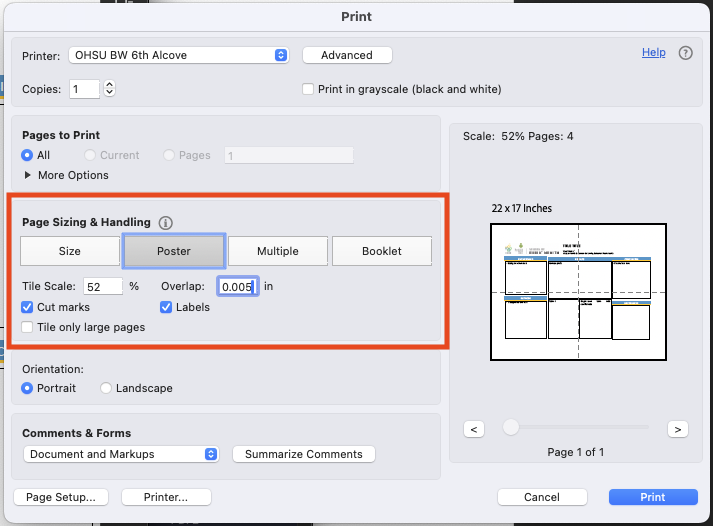
\includegraphics[keepaspectratio]{../project/images/poster_printing.png}}
  \item
    Choose the poster print option then choose the appropriate Tile
    Scale to make the poster span 4 pages
  \item
    Note: not all printers accommodate this
  \end{itemize}
\end{itemize}

\begin{tcolorbox}[enhanced jigsaw, arc=.35mm, bottomrule=.15mm, bottomtitle=1mm, breakable, colback=white, colbacktitle=quarto-callout-note-color!10!white, colframe=quarto-callout-note-color-frame, coltitle=black, left=2mm, leftrule=.75mm, opacityback=0, opacitybacktitle=0.6, rightrule=.15mm, title=\textcolor{quarto-callout-note-color}{\faInfo}\hspace{0.5em}{Note}, titlerule=0mm, toprule=.15mm, toptitle=1mm]

\begin{itemize}
\tightlist
\item
  Printing in Vanport is still a little dicey, so if you have access to
  a printer that can print posters, I would recommend using that
\item
  \textbf{Posters presented on 6/8 in class do NOT need to be what you
  turn in on 6/9 at 11pm in Sakai}
\end{itemize}

\end{tcolorbox}

\paragraph{Tables and figures}\label{tables-and-figures}

\begin{itemize}
\tightlist
\item
  Tables and figures should NOT have variable names as they appear in
  the data frame

  \begin{itemize}
  \tightlist
  \item
    Variable names should be understood by a reader
  \item
    Variable names should be written in full words
  \item
    Include a title or caption for all figures
  \item
    Figure and tables appear on same page or close to same page where
    they are first referenced
  \item
    Tables and figures are an appropriate size in the html
  \item
    Nicky is able to read all words in figures and tables
  \end{itemize}
\item
  Figures and tables should be clear and crisp

  \begin{itemize}
  \tightlist
  \item
    Make sure they are not blurred
  \item
    Screenshots are okay, but will likely make them blurry if you're not
    careful
  \item
    Best option is to use the \texttt{save()} to save a jpg or png
  \end{itemize}
\end{itemize}

\paragraph{Writing}\label{writing}

\begin{itemize}
\tightlist
\item
  Writing, spelling, and grammar should be admissible

  \begin{itemize}
  \tightlist
  \item
    This means I can generally follow your thought/what you are trying
    to communicate
  \item
    Some spelling and grammar mistakes are allowed

    \begin{itemize}
    \tightlist
    \item
      I will not take off points if there are a few sprinkled in
    \item
      If \emph{every or close to every} sentence has mistakes, then I
      will take off
    \end{itemize}
  \end{itemize}
\end{itemize}

\subsubsection{Poster template}\label{poster-template}

\begin{itemize}
\tightlist
\item
  \href{https://ohsuitg-my.sharepoint.com/:p:/r/personal/wakim_ohsu_edu/Documents/Teaching/Classes/BSTA_513_26S/Student_files_BSTA_513/Project/Resources/poster_template.pptx?d=wb113c78c33e4497fab393030df6448e6&csf=1&web=1&e=2STsp5}{Powerpoint
  Template}

  \begin{itemize}
  \tightlist
  \item
    Feel free to adjust this poster visually
  \end{itemize}
\end{itemize}

\subsubsection{Poster examples}\label{poster-examples}

\begin{itemize}
\tightlist
\item
  \href{https://ohsuitg-my.sharepoint.com/:b:/r/personal/wakim_ohsu_edu/Documents/Teaching/Classes/BSTA_513_26S/Student_files_BSTA_513/Project/Sample_poster/McVeety_Trans_Single_Payer_Poster.pdf?csf=1&web=1&e=L77P3h}{Poster
  1}

  \begin{itemize}
  \tightlist
  \item
    Good example of layouts and well-executed visuals
  \end{itemize}
\item
  \href{https://ohsuitg-my.sharepoint.com/:b:/r/personal/wakim_ohsu_edu/Documents/Teaching/Classes/BSTA_513_26S/Student_files_BSTA_513/Project/Sample_poster/Analysis\%20of\%20Veterans\%27\%20Non-disclosure\%20of\%20Suicidal\%20Thoughts.pdf?csf=1&web=1&e=MTVk2f}{Poster
  2}

  \begin{itemize}
  \tightlist
  \item
    Good example of a forest plot to display coefficient estimates of
    many covariates
  \item
    Good example of patient information displayed
  \item
    Good highlight of the study goals in the background
  \end{itemize}
\item
  \href{https://ohsuitg-my.sharepoint.com/:b:/r/personal/wakim_ohsu_edu/Documents/Teaching/Classes/BSTA_513_26S/Student_files_BSTA_513/Project/Sample_poster/nwakim_prop_score.pdf?csf=1&web=1&e=rN4Sry}{Poster
  3}

  \begin{itemize}
  \tightlist
  \item
    Done by Nicky (a long time ago) so please excuse a lot of the poor
    language around race/ethnicity

    \begin{itemize}
    \tightlist
    \item
      I have learned a lot since then! My statistics education did not
      do a great job of incorporating responsible practice around
      participant's identities
    \end{itemize}
  \item
    Showing this poster because it is a good example of the level of
    detail expected in our poster's background, methods, and conclusions
  \end{itemize}
\item
  \href{https://ohsuitg-my.sharepoint.com/:f:/r/personal/wakim_ohsu_edu/Documents/Teaching/Classes/BSTA_513_26S/Student_files_BSTA_513/Project/Sample_poster?csf=1&web=1&e=eBBVb4}{More
  posters can be found in our shared folder}
\end{itemize}

\subsubsection{Grading}\label{grading}

The project report is out of 36 points. Note that the Statistical
Methods and Results sections are graded on an 8-point scale, while all
other components are graded on a 4-point scale.

\href{https://ohsuitg-my.sharepoint.com/:x:/r/personal/wakim_ohsu_edu/Documents/Teaching/Classes/BSTA_513_26S/Student_files_BSTA_513/Project/Resources/Project_Rubric_513_613_26S.xlsx?d=w5ebea0e980ee4149a3897e923c866a0d&csf=1&web=1&e=CGg89t}{Please
see the excel spreadsheet if you would like to check if you have all the
needed components for the poster!}

\begin{itemize}
\tightlist
\item
  Example: In the Formatting Section, a check mark for ``With little
  editing, the poster can be presented at a conference'' means that the
  poster has zero (or some) grammar or spelling mistakes, no code chunks
  showing, and no output warnings nor messages showing.
\item
  Professional figures mean

  \begin{itemize}
  \tightlist
  \item
    I can read the words and numbers in the html

    \begin{itemize}
    \tightlist
    \item
      Variable names are converted from the data frame version to
      readable text
    \item
      For example: \texttt{iam\_001} does not show up on axes, instead
      something like: \texttt{Response\ to\ "Currently,\ I\ am..."}
    \end{itemize}
  \item
    Colors are only used if conveying information
  \item
    Intended message of the figure is easily understood

    \begin{itemize}
    \tightlist
    \item
      If you are trying to show a trend of mean IAT vs.~an ordered
      categorical variable, then the variable is ordered on the x-axis
    \end{itemize}
  \end{itemize}
\item
  For the references

  \begin{itemize}
  \tightlist
  \item
    I will not be overly critical about the formatting
  \item
    By consistency, I mean that you if you are citing things like (Last
    Name, Year) it doesn't suddenly change to number citations.
  \item
    If you would like to use Quarto's citation tool, you can! I actually
    pair it with Zotero and it works beautifully! (But I would not
    embark on this if you haven't used Zotero before)
  \end{itemize}
\item
  EXTRA CREDIT for

  \begin{itemize}
  \tightlist
  \item
    \href{https://forms.office.com/Pages/ResponsePage.aspx?id=V3lz4rj6fk2U9pvWr59xWFMopmPUjRtDiHLswhgacNhUMzU0RkJVVThPNFZZUERNSkdWVlBBWTdEWCQlQCNjPTEu}{Bringing
    food/drink etc. to the Poster Day!}
  \item
    \href{https://forms.office.com/Pages/ResponsePage.aspx?id=V3lz4rj6fk2U9pvWr59xWFMopmPUjRtDiHLswhgacNhUQ1E0UDQ2QUhSRkpPV0JOMzY5TFA0QTUyMSQlQCNjPTEu}{Completing
    the course eval!}
  \end{itemize}
\end{itemize}

\subsection{Sections}\label{sections}

\subsubsection{Title}\label{title}

\begin{itemize}
\tightlist
\item
  \textbf{Purpose:} Create an identifiable name for your research
  project
\item
  IF you did {purposeful model selection}, this should emphasize that
  you are focusing on the relationship between your explanatory variable
  and food insecurity
\item
  If you did {LASSO}, this should emphasize that you are focusing on
  predicting food insecurity and what variables can predict it
\end{itemize}

\subsubsection{Introduction/Background}\label{introductionbackground}

\begin{itemize}
\tightlist
\item
  \textbf{Length: 5-8 bullets}
\item
  \textbf{Purpose:} Introduce the research question and why it is
  important to study
\item
  This section is non-technical.

  \begin{itemize}
  \tightlist
  \item
    By reading just the introduction and conclusion, someone without a
    technical background should have an idea of what they study was
    about, why it is important, and what the main results are
  \end{itemize}
\item
  You may start with your bullets from Lab 1, but you should edit it and
  make sure it flows into your report well!
\item
  This should hit on three main points:

  \begin{itemize}
  \tightlist
  \item
    What is the context of this research? What is going in the world or
    public health sector that has led us to study this outcome? Why is
    the outcome important to study?
  \item
    Required for {purposeful model selection}, but not for LASSO:What is
    the relationship between your explanatory variable and the outcome?
    Why is this relationship important to study?

    \begin{itemize}
    \tightlist
    \item
      What prior research leads us to our research question?
    \end{itemize}
  \item
    What is your guiding question?

    \begin{itemize}
    \tightlist
    \item
      Best if this comes last in the introduction
    \item
      Helpful if you highlight this for your audience
    \item
      If you perform {LASSO}, it would be good to mention prediction
      here
    \end{itemize}
  \end{itemize}
\item
  The intro should start broad and get more focused towards the end
\item
  Should contain some references
\end{itemize}

\subsubsection{Methods}\label{methods}

\begin{tcolorbox}[enhanced jigsaw, arc=.35mm, bottomrule=.15mm, bottomtitle=1mm, breakable, colback=white, colbacktitle=quarto-callout-caution-color!10!white, colframe=quarto-callout-caution-color-frame, coltitle=black, left=2mm, leftrule=.75mm, opacityback=0, opacitybacktitle=0.6, rightrule=.15mm, title=\textcolor{quarto-callout-caution-color}{\faFire}\hspace{0.5em}{Caution}, titlerule=0mm, toprule=.15mm, toptitle=1mm]

Think of this section as the \textbf{HOW: How did you approach your
research question?}

How did you analyze the data? How did you select variables for your
model? How did you check diagnostics?

\end{tcolorbox}

\begin{itemize}
\tightlist
\item
  \textbf{Length: 8-10 bullets}
\item
  \textbf{Purpose:} Describe the analyses that were conducted and
  methods used to select variables and check diagnostics
\item
  \textbf{Some important methods to discuss} (You may divide these into
  your sections, not necessarily with these names)

  \begin{itemize}
  \tightlist
  \item
    General approach to the dataset

    \begin{itemize}
    \tightlist
    \item
      2-3 bullets
    \item
      Where did the data come from?
    \item
      Did you need to do any quality control?
    \item
      Missing data: we performed complete case analysis

      \begin{itemize}
      \tightlist
      \item
        1 bullet
      \end{itemize}
    \item
      What program did you use to analyze the data?
    \end{itemize}
  \item
    Variables and variable creation

    \begin{itemize}
    \tightlist
    \item
      {For purposeful model selection}: This includes a description of
      analyses for Table 1 and what statistics were used to summarize
      the variables

      \begin{itemize}
      \tightlist
      \item
        More on creation of Table 1, not discussing the results of Table
        1
      \end{itemize}
    \item
      Includes (only include if you did one of the following)

      \begin{itemize}
      \tightlist
      \item
        Categorizing a continuous variable (even if performed in model
        selection)
      \item
        Using scoring for an ordered categorical variable
      \item
        Moving categories around or combining categories
      \item
        Potential examples:

        \begin{itemize}
        \tightlist
        \item
          We categorized age into the following groups: \_\_\_,
          \_\_\_\_, \_\_\_\_, \_\_\_\_ based on existing guidelines from
          \textless insert reference here\textgreater.
        \item
          We created a new variable for any hardship by combining the
          following variables: \_\_\_, \_\_\_, and \_\_\_. We
          categorized this variable into the following groups: \_\_\_,
          \_\_\_, and \_\_\_
        \item
          We treated number of children as numeric
        \end{itemize}
      \end{itemize}
    \item
      1 bullet for all variables
    \end{itemize}
  \item
    Model building: we performed {purposeful model selection} OR {LASSO}

    \begin{itemize}
    \tightlist
    \item
      1-3 bullets
    \item
      {For purposeful model selection}, this includes

      \begin{itemize}
      \tightlist
      \item
        Describe purposeful selection: combining existing literature,
        clinical significance, and analysis
      \item
        How did you build the model? Describe the process
      \item
        Did you consider confounders and effect modifiers?
      \item
        Example: We considered the following potential confounders: list
        fo them. Based on our research question, existing literature,
        and clinical significance, we used purposeful selection to
        identify confounders and effect modifiers.
      \end{itemize}
    \item
      {For LASSO}, this includes

      \begin{itemize}
      \tightlist
      \item
        Percent split for training and testing data
      \item
        Did you tune your penalty? What was the value of your penalty?
      \item
        Did you use cross-validation?
      \item
        What variables did you exclude from consideration from LASSO?
      \end{itemize}
    \end{itemize}
  \item
    {For purposeful model selection}: Final model

    \begin{itemize}
    \tightlist
    \item
      1 bullet
    \item
      \textbf{Only for {purposeful model selection}!!}

      \begin{itemize}
      \tightlist
      \item
        In {LASSO}, the final model is more of a result
      \end{itemize}
    \item
      Write out your final model: It can be an equation, but a list
      might be nicer.

      \begin{itemize}
      \tightlist
      \item
        Example: Our final model included main effects for \_\_\_\_ and
        an interaction between \_\_ and \_\_.
      \end{itemize}
    \end{itemize}
  \item
    Model diagnostics

    \begin{itemize}
    \tightlist
    \item
      1-2 bullets
    \item
      Includes

      \begin{itemize}
      \tightlist
      \item
        Process of investigating model diagnostics
      \end{itemize}
    \end{itemize}
  \end{itemize}
\end{itemize}

\begin{tcolorbox}[enhanced jigsaw, arc=.35mm, bottomrule=.15mm, bottomtitle=1mm, breakable, colback=white, colbacktitle=quarto-callout-caution-color!10!white, colframe=quarto-callout-caution-color-frame, coltitle=black, left=2mm, leftrule=.75mm, opacityback=0, opacitybacktitle=0.6, rightrule=.15mm, title=\textcolor{quarto-callout-caution-color}{\faFire}\hspace{0.5em}{Important to keep in mind}, titlerule=0mm, toprule=.15mm, toptitle=1mm]

Methods typically describe your approach and process, not the results of
that process

\begin{itemize}
\tightlist
\item
  For example: I might say ``We investigated the linearity of each
  continuous covariate visually. If continuous variables were not
  linear, then we divided the variable into categories using existing
  guidelines from \textless insert reference here\textgreater{} or
  creating quartiles.''
\item
  In the methods section, I would NOT say: ``We investigated the
  linearity of each continuous covariate visually. We found that age was
  not linearly related to IAT scores. Thus, we categorized age into the
  following groups: \_\_\_, \_\_\_\_, \_\_\_\_, \_\_\_\_, and
  \_\_\_\_.''
\item
  The last two sentences about age would be more appropriate in the
  Results section
\end{itemize}

\end{tcolorbox}

\subsubsection{Results}\label{results}

\begin{tcolorbox}[enhanced jigsaw, arc=.35mm, bottomrule=.15mm, bottomtitle=1mm, breakable, colback=white, colbacktitle=quarto-callout-caution-color!10!white, colframe=quarto-callout-caution-color-frame, coltitle=black, left=2mm, leftrule=.75mm, opacityback=0, opacitybacktitle=0.6, rightrule=.15mm, title=\textcolor{quarto-callout-caution-color}{\faFire}\hspace{0.5em}{Caution}, titlerule=0mm, toprule=.15mm, toptitle=1mm]

Think of this section as the \textbf{WHAT: What did you find?}

What were the results of your analyses? What do the numbers mean (not
mean like their context, but mean like direct interpretations)? What are
the important trends in the data?

\end{tcolorbox}

\begin{itemize}
\tightlist
\item
  \textbf{Length: mostly figures with 3-4 bullet points}
\item
  \textbf{Purpose:} Relay the results from our sample's analysis
  typically focusing on the numbers and interpretations
\item
  Tables \& figures (2-3 tables or figures)

  \begin{itemize}
  \tightlist
  \item
    The following are required tables or figures

    \begin{itemize}
    \tightlist
    \item
      Table 1 summarizing participant characteristics

      \begin{itemize}
      \tightlist
      \item
        If LASSO, use the top 10 important variables
      \end{itemize}
    \item
      If {purposeful model selection}: Table or figure with regression
      results

      \begin{itemize}
      \tightlist
      \item
        Can be a forest plot
      \item
        If you have A LOT of coefficient estimates, the forest plot may
        not work well!
      \end{itemize}
    \item
      If {LASSO}: table or figure with variable importance
    \end{itemize}
  \item
    \textbf{1-2 figures that you think are helpful in understanding the
    results, for example}

    \begin{itemize}
    \item
      DAG explaining connection between variables (if you did this)
    \item
      Figure for the AUC-ROC
    \item
      Table or figure to compare model fit statistics (if you did this)
    \item
      Table or figure for unadjusted relationship between outcome and
      explanatory variables
    \end{itemize}
  \end{itemize}
\item
  {For purposeful model selection:} Interpret the \textbf{important}
  model coefficients in the context of the research question

  \begin{itemize}
  \tightlist
  \item
    3-4 bullets
  \item
    Interpreting the explanatory variable's relationship with IAT score
    is the most important thing to report!!

    \begin{itemize}
    \tightlist
    \item
      When doing this, make sure you account for ALL interactions: If
      your explanatory variable has multiple interactions and you are
      trying to interpret one, then what does that mean about the other
      variables involved in the other interactions? If this is
      confusing, please make an appointment with me!!
    \end{itemize}
  \end{itemize}
\item
  {For LASSO:} Discuss the important variables and identify the 1-3 most
  important ones

  \begin{itemize}
  \tightlist
  \item
    3-4 bullets
  \item
    Since our main focus is prediction, we want to discuss variables
    that most contribute to the prediction of the outcome
  \item
    Other interesting trends might include variables that you thought
    would be important but were not, or variables that you thought would
    not be important but were

    \begin{itemize}
    \tightlist
    \item
      Were there correlated variables that were important?
    \end{itemize}
  \end{itemize}
\end{itemize}

\subsubsection{Conclusion/Discussion}\label{conclusiondiscussion}

\begin{tcolorbox}[enhanced jigsaw, arc=.35mm, bottomrule=.15mm, bottomtitle=1mm, breakable, colback=white, colbacktitle=quarto-callout-caution-color!10!white, colframe=quarto-callout-caution-color-frame, coltitle=black, left=2mm, leftrule=.75mm, opacityback=0, opacitybacktitle=0.6, rightrule=.15mm, title=\textcolor{quarto-callout-caution-color}{\faFire}\hspace{0.5em}{Caution}, titlerule=0mm, toprule=.15mm, toptitle=1mm]

Think of this section as the \textbf{WHY: Why did we get these results?}

Why are they important? Why are they relevant (or not) to the target
population? Why might we use these results? Why might we not use these
results? Why are they limited (and what are the consequences of those
limitations)?

\end{tcolorbox}

\begin{itemize}
\tightlist
\item
  \textbf{Length: 5-10 bullets}
\item
  \textbf{Purpose:} Describe the main conclusions to a non-technical
  audience and discuss the results and give them context outside of the
  sample and its analysis
\item
  {For purposeful model selection:} What was the answer to your research
  question?

  \begin{itemize}
  \tightlist
  \item
    Mention the direction of the association if there was one
  \end{itemize}
\item
  {For LASSO:} What was the biggest predictor of food insecurity?

  \begin{itemize}
  \tightlist
  \item
    Did your original variable of interest have any importance?
  \end{itemize}
\item
  Any other interesting results?
\item
  Some important things to include

  \begin{itemize}
  \tightlist
  \item
    Include limitations and consequences of the limitations on the
    results

    \begin{itemize}
    \tightlist
    \item
      You don't need to hit all the limitations, but think about the big
      ones (generalizability? independence of samples? large sample size
      vs.~clinical significance? the way we handled variables?)
    \item
      A REALLY big limitation of this analysis is that we used survey
      data, but did not use survey weights. This means we might have
      biased results that are not generalizable to the US population.
    \end{itemize}
  \item
    After limitations, discuss the positive parts of the results

    \begin{itemize}
    \tightlist
    \item
      What can we do with these results? What impact can it have?
    \end{itemize}
  \item
    Any overarching trends that are worth noting?
  \end{itemize}
\item
  Should contain some references
\end{itemize}

\subsubsection{References}\label{references}

\begin{itemize}
\tightlist
\item
  Include your references here!
\item
  You introduction should have references, especially when discussing
  the social science behind the analysis
\item
  You must reference the WBNS data source!!
\end{itemize}




\end{document}
